%%%%%%%%%%%%%%%%%%%%%%%%%%%%%%%%%%%%%%%%%
% This is the LaTeX template of Jonas Schultheiss. It'll be used for the IPA and VA.
% 
% This template can be downloaded here:
% https://github.com/
% 
% This template is heavily inspired by Marco Roth's template:
% https://github.com/marcoroth
%
% Template license:
% MIT
% https://github.com/jonasschultheiss/LaTeX-Template/blob/master/LICENSE
% ./LICENSE
%%%%%%%%%%%%%%%%%%%%%%%%%%%%%%%%%%%%%%%%%

%%%%%%%%%%%%%%%%%%%%%%
% Document & Variables
%%%%%%%%%%%%%%%%%%%%%%

\documentclass[10pt, oneside]{scrbook}

\newcommand{\version}{0.1.5}
\newcommand{\docdate}{\today}
\newcommand{\docname}{OSE Dashboard}
\newcommand{\compiledfilename}{ipa\_jsc\_ose\_2021.pdf}
\newcommand{\task}{Individuelle praktische Arbeit} % e.g. Modul 152/IPA/...
\newcommand{\taskname}{3D Web Anwendung des OSE Modells für die Produktion vorbereiten}
\newcommand{\clientlogopath}{./images/eh-logo.png}
\newcommand{\kandidat}{Jonas Schultheiss}
\newcommand{\fachkraft}{Markus Strittmatter}
\newcommand{\hauptexperte}{Matthias Meier}
\newcommand{\nebenexperte}{Jens Schwyn Aerni}
\newcommand{\docauthor}{\kandidat}

%%%%%%%%%%
% Packages
%%%%%%%%%%

\usepackage[
  a4paper,
  left=25mm,
  right=25mm,
  top=35mm,
  bottom=35mm,
  headheight=35mm
]{geometry}
\usepackage[utf8]{inputenc}
\usepackage[babel,german=swiss]{csquotes}
\usepackage[ngerman]{babel}
\usepackage[printonlyused]{acronym}
\usepackage[section]{placeins}
\usepackage[Conny]{fncychap}
\usepackage[T1]{fontenc}
\usepackage[T1]{fontenc}
\usepackage[table]{xcolor}
\usepackage{caption}
\usepackage{color}
\usepackage{fancyhdr}
\usepackage{graphics}
\usepackage{graphicx}
\usepackage{helvet}
\usepackage{lastpage}
\usepackage{lipsum}
\usepackage{listings}
\usepackage{multicol}
\usepackage{multirow}
\usepackage{parskip}
\usepackage{pdfpages}
\usepackage{pifont}
\usepackage{tabularx}
\usepackage{tocloft}
\usepackage{xurl}
\usepackage{wrapfig}
\usepackage{xcolor}
\usepackage{afterpage}
\usepackage[backend=biber, style=numeric]{biblatex}
\usepackage{suffix}
\usepackage{float}

%%%%%%%%
% Colors
%%%%%%%%

\definecolor{lightgray}{RGB}{224,224,224}
\definecolor{darkgray}{RGB}{192,192,192}

\renewcommand{\listfigurename}{List of figures}


%%%%%%%%%%%%%%%%%%%
% Headers & Footers
%%%%%%%%%%%%%%%%%%%

\pagestyle{fancy}
\renewcommand{\chapterpagestyle}{fancy}
\renewcommand{\partpagestyle}{fancy}
\fancyhead{}
\fancyhead[R]{\fontsize{10}{12} \selectfont \textbf{\task} \\ \fontsize{8}{10} \selectfont \taskname \\ Kandidat: \docauthor}
\fancyhead[L]{\includegraphics[width=6cm]{\clientlogopath}}
\fancyfoot{}
\fancyfoot[L]{\fontsize{10}{11} \selectfont \compiledfilename}
\fancyfoot[C]{\fontsize{9}{11} \docdate}
\fancyfoot[R]{\fontsize{10}{11} \selectfont Seite \thepage\ von \pageref{LastPage}}

\renewcommand{\headrulewidth}{0pt}

%%%%%%
% Font
%%%%%%

\renewcommand{\familydefault}{\sfdefault}

%%%%%
% TOC
%%%%%

\renewcommand{\cftchapafterpnum}{\vspace{5pt}}

%%%%%
% LOF
%%%%%

\captionsetup{justification=centering}

%%%%%%%%%%
% Graphics
%%%%%%%%%%

\setcounter{totalnumber}{5}
\ChNumVar{\Huge}
\ChTitleVar{\huge\sffamily}
\ChNameVar{\large\sffamily}
\ChRuleWidth{0.5pt}

%%%%%%%%%%%%%%
% Line spacing
%%%%%%%%%%%%%%

\renewcommand{\baselinestretch}{1,3}

%%%%%%%%%%%%%%%%
% PDF formatting
%%%%%%%%%%%%%%%%

\definecolor{codegray}{gray}{0.9}
\newcommand{\code}[1]{\colorbox{codegray}{\texttt{#1}}}
\usepackage[
  bookmarks=true,           % Lesezeichen erzeugen
  bookmarksopen=true,       % Lesezeichen ausgeklappt
  bookmarksnumbered=true,   % Anzeige der Kapitelzahlen
  breaklinks=true,          % Ermöglicht einen Umbruch von URLs
  colorlinks=true,          % Einfärbung von Links
  linkcolor=black,          % Linkfarbe: schwarz
  anchorcolor=black,        % Ankerfarbe: schwarz
  citecolor=black,          % Literaturlinks: schwarz
  filecolor=black,          % Links zu lokalen Dateien: schwarz
  menucolor=black,          % Acrobat Menü Einträge: schwarz
  urlcolor=black,           % URL-Farbe: schwarz
  pdftitle={OSEDashboard},
  pdfauthor={Jonas Schultheiss},
  pdfsubject={OSEDashboard},
  pdfkeywords={OSE, OSEDashboard, Dashboard, ipa, jonas, schultheiss}
]{hyperref}

%%%%%%%%%%%%%%
% Reset indent
%%%%%%%%%%%%%%

\setlength{\parindent}{0pt}

%%%%%%%%%
% Columns
%%%%%%%%%

\setlength{\columnseprule}{1pt}
\def\columnseprulecolor{\color{black}}

%%%%%%%%%%%%%
% Titel fonts
%%%%%%%%%%%%%

\newcommand{\titlesize}{\fontsize{25pt}{20pt}\selectfont}
\newcommand{\subtitlesize}{\fontsize{15pt}{10pt}\selectfont}
\newcommand{\subsubtitlesize}{\fontsize{10pt}{5pt}\selectfont}
\addbibresource{quellen.bib}
\AtBeginDocument{\addtocontents{toc}{\protect\thispagestyle{fancy}}} 

\begin{document}
  \begin{titlepage}
  \centering
  \titlesize{\textbf{\task}}
  \linebreak
  \linebreak
  \linebreak
  \linebreak
  \linebreak
  \linebreak
  \linebreak
  \linebreak
  \linebreak
  \linebreak
  \linebreak
  \subtitlesize{\textbf{\taskname}}
  \linebreak
  \linebreak
  \linebreak
  \linebreak
  \subtitlesize{\docdate}
  \linebreak
  \linebreak
  \linebreak
  \linebreak
  \linebreak
  \linebreak
  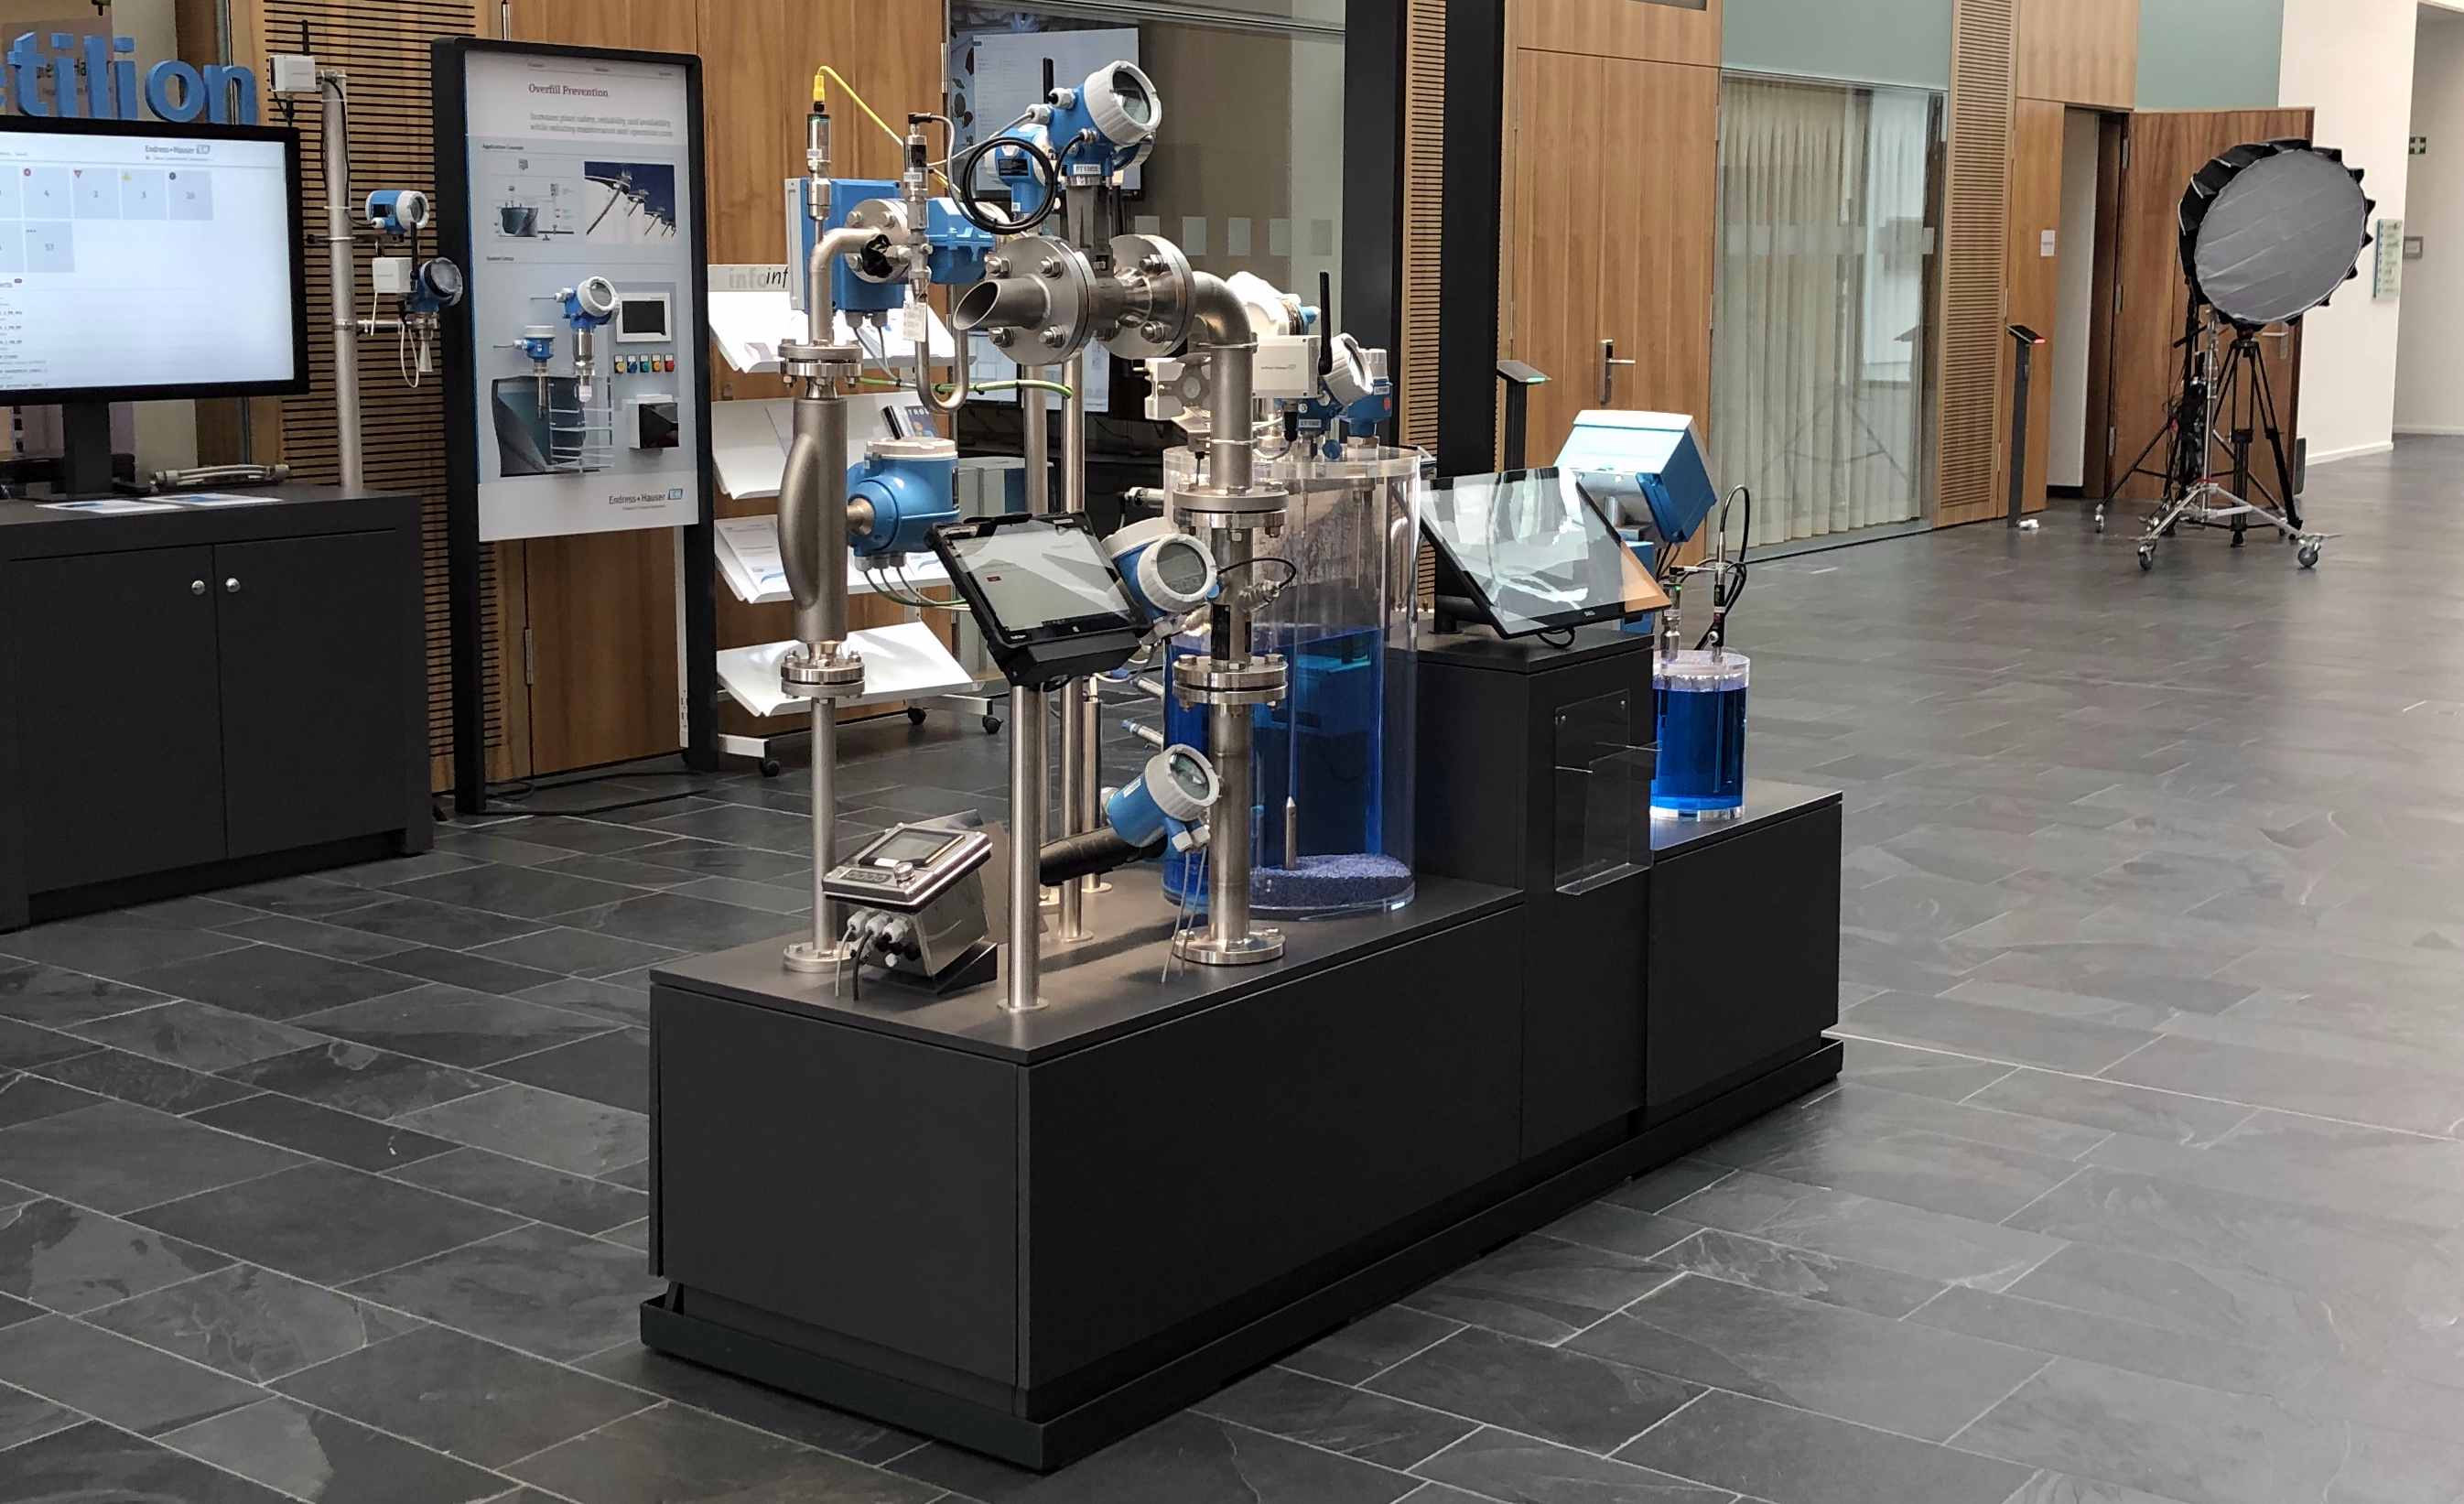
\includegraphics[width=0.85\textwidth]{./images/OSEModel.png}
  \linebreak
  \linebreak
  \linebreak
  \linebreak
  \linebreak
  \linebreak
  \linebreak
  \linebreak
  \linebreak
  \linebreak
  \linebreak
  \linebreak
  \linebreak
  \linebreak
  \linebreak
  \linebreak
  \linebreak
  \linebreak
  \linebreak
  \linebreak
  \linebreak
  \linebreak
  \subsubtitlesize{\textbf{Version: \version}}
  \linebreak
  \linebreak
  \subsubtitlesize{\textbf{Durchführung:} 29.03.2021 - 14.04.2021}
  \linebreak
  \begin{multicols}{2}
    \begin{flushright}
      \subsubtitlesize{\textbf{Verantwortliche Fachkraft}}\hspace*{1cm}
      \linebreak
      \subsubtitlesize{\fachkraft}\hspace*{1cm}
      \linebreak
      \subsubtitlesize{markus.strittmatter@endress.com}\hspace*{1cm}
      \linebreak
      \linebreak
      \subsubtitlesize{\textbf{Hauptexperte}}\hspace*{1cm}
      \linebreak
      \subsubtitlesize{\hauptexperte}\hspace*{1cm}
    \end{flushright}
    \begin{flushleft}
      \hspace*{1cm}\subsubtitlesize{\textbf{Kandidat}}
      \linebreak
      \hspace*{1cm}\subsubtitlesize{\kandidat}
      \linebreak
      \hspace*{1cm}\subsubtitlesize{jonas.schultheiss@endress.com}
      \linebreak
      \linebreak
      \hspace*{1cm}\subsubtitlesize{\textbf{Nebenexperte}}
      \linebreak
      \hspace*{1cm}\subsubtitlesize{\nebenexperte}
      \end{flushleft}
    \end{multicols}
\end{titlepage}

  \frontmatter
  \pagenumbering{Roman}
  \chapter*{Dokumentmanagement}
\vspace{-3cm}
\begin{table}[htp]
  \begin{tabularx}{\textwidth}{l X}
  Autor: & Jonas Schultheiss \\
  Version: & \version \\
  Datum: & \docdate \\
  Status: & In Progress \\
  Dateiname: & \compiledfilename \\
  \end{tabularx}
\end{table}

\begin{table}[htp]
  \begin{tabularx}{\textwidth}{l l X}\hline \\
  \textbf{Version} & \textbf{Datum} & \textbf{Änderung} \\ \\\hline \\
  0.0.1 & 29.03.2021 & Initialisierung des Dokuments \\
  0.0.2 & 29.03.2021 & Projektmanagementmethode beschrieben \\
  \\\hline
  \end{tabularx}
\end{table}

  \chapter*{Danksagung}
\vspace{-3cm}
Zunächst möchte ich Markus Strittmatter und Endress+Hauser für diese Ausbildung danken. Nur durch Sie konnte ich in den letzten vier Jahren meine Leidenschaft und mein Können für das Programmieren weiterentwickeln. Dafür bin ich froh, da ich nun weiss, dass Informatik das Richtige für mich ist. Es ist auch nicht selbstverständlich, einen Lehrling die Fachrichtung wechseln zu lassen. Dies erlaubte mir mich auch in der Schule voll und ganz auf das Programmieren zu fokussieren.
\newline
\newline
Gerne würde ich mich auch bei Valentino Rusconi und Marco Roth bedanken. Konnte ich etwas nicht alleine bewältigen, nahmen Sie sich die Zeit, um mir komplexe Konzepte zu erklären oder bei schwierigen Fehlern zu helfen.
\newline
\newline
Abschliessend möchte ich mich auch recht herzlich bei Lisa Marie Hüglin, Robert Kölblin und Simon Jäggi für das Korrekturlesen bedanken.
  \chapter*{Kurzfassung}
\vspace{-3cm}
\section*{Ausgangssituation}

\lipsum[2-4][12-18]

\section*{Umsetzung}

\lipsum[2-4][12-18]

\section*{Ergebnis}

\lipsum[2-4][12-18]
  \tableofcontents
  \mainmatter
  \pagestyle{fancy}
  \part{Obligatorische Kapitel}
  \chapter{Obligatorische Dokumentation}
\section{Ausgangslage}

In der Endress+Hauser Gruppe gibt es ein Messemodell mit dem Namen One Story Exhibit (OSE Modell). Dieses OSE Modell gibt es mehrfach in der gleichen Ausführung. Diese Modelle sind weltweit in den Endress+Hauser Sales Center verteilt. Dieses Modell bietet einen interaktiven Einblick in das Produkt Portfolio von Endress+Hauser Digital Solutions. Der Kunde kann unter anderem unser IIOT Angebot Netilion interaktiv erleben. Aktuell werden dafür unsere Netilion Standard Services wie z.B. Analytics, Health und Value verwendet. Dabei werden die Daten der Messgeräte via Edge Device in unserer IIOT Cloud gespeichert. Via Netilion Standard Web Applikationen kann man z.B. den aktuellen Health Status der Messgeräte sowie den aktuellen Messwert sehen.
\newline
\newline
Die Web Applikation „OSE Dashboard“ soll dem Kunden ein Beispiel für die Verwendung der Netilion Connect Subscription zeigen. Mit einer Netilion Connect Subscription erhält der Kunde Zugriff auf die REST API unserer Netilion Cloud und kann somit eigene IIOT Anwendungen entwickeln oder die Daten aus Netilion in seine eigene Cloud importieren. Die Applikation „OSE Dashboard“ zeigt das OSE Modell in einer 3D Ansicht. Man kann über eine Kameraführung an die Messgeräte heran zoomen und den Health Status des Messgerätes anzeigen lassen. Aktuell ist die Applikation nur mit dem OSE Modell in Reinach nutzbar, weil die Applikation nur mit den Daten der Messgeräte dieses Modells in Netilion verlinkt ist.
\newline
Mit dieser IPA soll die Web Applikation „OSE Dashboard“ so erweitert werden, dass sie für andere OSE Modelle mit gleichem Aufbau verwendet werden kann.
\section{Detaillierte Aufgabenstellung}

Die bestehende Web Anwendung „OSE Dashboard“ zeigt das One Story Exhibit Model (OSE Modell), welches in Reinach steht, in einer 3D Ansicht an. Darin werden die Daten der Messgeräte aus der Netilion Cloud gelesen und ebenfalls dargestellt.
\newline
Das Ziel dieses Projekts ist, dass die Web Anwendung auch für andere OSE Modelle, welche dem gleichen Aufbau haben, verwendet werden kann, ohne dass zukünftig eine Änderung an der Applikation notwendig ist.
\newline
Die bestehende Anwendung muss dafür so erweitert werden, dass Verlinkung des 3D Modells mit den Daten der Messgeräte nicht mehr im Source Code hinterlegt ist. Es muss ein Weg gefunden werden, diese Verlinkung für alle bestehenden und zukünftigen OSE Modelle zu speichern.
\newline
Laut Autraggeber haben alle OSE Modelle den gleichen Aufbau mit Messgeräten vom gleichen Typ. Auch die Bezeichnung der Messgeräte sollte bei allen Modellen gleich sein. Wird die Anwendung das erste mal für ein OSE Modell verwendet, muss für alle Geräte aus diesem OSE Modell die Verlinkung mit dem 3D Modell der Anwendung automatisch erfolgen und gespeichert werden. Sollte es aber Messgeräte geben, die nicht vom gleichen Typ sind, weil sie z.B. durch eine neuere Version ersetzt wurden, dann soll der Anwender die Möglichkeit haben über ein Konfigurationsmenü die Verlinkung vorzunehmen.
\newline
Änderungen an der Konfiguration dürfen nicht von jedem User vorgenommen werden. Das Konfigurationsmenü darf nur von Usern geöffnet werden, welche die entsprechende Berechtigung haben. Dafür soll in Netilion eine User Gruppe erstellt werden. Alle User dieser Gruppe dürfen dann die Konfiguration ändern.
\newline
Die Anwendung selber soll aber weiterhin ohne Login aufrufbar sein. Der Anwender soll als Datenquelle für das 3D Modell zwischen den verschiedenen integrierten Standorten wählen können. Da jedes OSE Modell einen eigenen User hat, müssen die User Credentials der einzelnen OSE Modelle ebenfalls in der Applikation gespeichert werden. Dabei muss darauf geachtet werden, dass diese Daten sicher gespeichert werden und der Anwender keinen Zugriff darauf hat.
\newline
Die Methoden mit der Logik für die automatische Verlinkung der Messgeräte mit dem 3D Modell soll automatisiert getestet werden.
\newline
Für den Test der kompletten Applikation sind manuelle Tests ausreichend. Dabei sind folgende Testsfälle zu beachten:
\begin{itemize}
  \item Konfigurationsmenu nur mit entsprechender Berechtigung aufrufbar
  \item Alle Messgeräte werden automatisch verlinkt.
  \item Messgeräte können nicht automatisch verlinkt werden .
  \item User kann ohne Login zwischen integrierten OSE Modellen wechseln.
  \item Credentials der OSE Modelle sind sicher gespeichert
\end{itemize}
Die Tests sollen zuerst an dem OSE Modell in Reinach durchgeführt werden. Bei diesem Modell können auch für Tests die Daten in Netilion mal abgeändert werden.
Zum Abschluss sollen 2 weitere OSE Modelle integriert werden um die funktionalität der Anwendung mit mehreren OSE Modellen zu testen.

\pagebreak
\section{Mittel und Methoden}
Anbei werden Mittel und Methoden aufgelistet, welche von diese IPA gefordert werden:
\begin{itemize}
  \item HTML \& CSS
  \item JavaScript
  \item Node.js JavaScript Runtime Environment für Desktop und Server
  \item React Eine von FaceBook entwickelte JavaScript Bibliothek, welche die Strukturierung von Komponenten basierten Benutzeroberflächen erleichtert.
  \item JSX Ein Syntax welcher das übliche JavaScript erweitert. Es ermöglicht das Vermischen von HTML mit JavaScript und wird
  von React verwendet
  \item Three JavaScript Bibliothek, welche es ermöglicht 3D Modelle in einem HTML Canvas darzustellen
  \item react-three-fiber JavaScript Bibliothek, welche auf Three aufbaut und das ganze in React verfügbar macht
  \item GLTF Dateiformat für 3D Modelle, welches sich am besten für das Web eignet
\end{itemize}

Hosting der Web Applikation
\begin{itemize}
  \item Heroku
  \item Vercel
\end{itemize}

Entwicklungsumgebung
\begin{itemize}
  \item Macbook Pro 2018 mit Dockingstation und 2 externen Monitoren. (Ersatzweise steht ein Windows Laptop zur Verfügung)
  \item MacOS Big Sur
  \item Visual Studio Code
  \item GitHub
\end{itemize}

\section{Vorkenntnisse}
Alle Tools und Techniken sind dem Lernenden schon bekannt. Er hat alle Tools, Programmiersprachen und Techniken schon in mehreren Projekten während der Ausbildung angewendet.

\section{Vorarbeiten}
Die Version 1 des OSE Dashboards wurde als Vorarbeit zu dieser IPA vom Lernenden entwickelt.

\section{Neue Lerninhalte}
In dieser IPA gibt es keine neuen Lerninhalte.

\section{Arbeiten in den letzten sechs Monaten}
Entwickeln einer Webanwendung, welche Daten aus der Endress+Hauser IIOT Plattform Netilion darstellt. Diese Anwendung zeigt den Wasserverbrauch der Kaffeemaschinen in der Pausenzone an und berechnet die Anzahl der konsumierten Tassen. Diese Anwendung dient dazu, unseren Kunden das Angebot Netilion Connect zu erklären.
\newline
Entwickeln einer weiteren Webanwendung, welche in Verbindung mit Netilion Connect Daten aus der Endress+Hauser IIOT Plattform darstellt. Dies ist die erste Version des OSE Dashboards, welches ein Messemodell in 3D darstellt und den „Gesundheitszustand“ der Messgeräte anzeigt. Diese Webanwendung wird im Rahmen dieser IPA erweitert.
\section{Projektaufbauorganisation}

\begin{figure}[!ht]
  \centering
  \includegraphics[width=.95\linewidth]{./images/Projektaufbauorganisation.png}
  \caption[Diagram der Projektaufbauorganisation]{Diagram der Projektaufbauorganisation}
  \label{fig:projektaufbauorganisation}
\end{figure}
\pagebreak
\section{Durchführungsblock}

\begin{table}[htp]
  \begin{tabularx}{\textwidth}{l X}
    Startblock 2: & 29.03.2021 – 16.04.2021\\
    PA-Durchführung: & 29.03.2021 – 14.05.2021 \\
    Einreichung bis: & 31.01.2021 \\
  \end{tabularx}
\end{table}

\section{IPA-Termine}

\begin{table}[htp]
  \begin{tabularx}{\textwidth}{l X}
    Antrittsgespräch: & 23.03.2021 08:30 \\
    Erster Zwischenbesuch: & 01.04.2021 09:00 \\
    Zweiter Zwischenbesuch: & 01.04.2021 00:00 \\
    Endbesuch: & 28.04.2021 09:00 \\
  \end{tabularx}
\end{table}
\section{Projektplan}
\includepdf[pages=-,pagecommand={},width=\textwidth, scale=0.8]{./projektplan/projektplan_ipa.pdf}
  \part{Dokumentation}
  \chapter{Projektmanagement}
\section{Entscheidung}
Die Entscheidung der Projektmanagementmethode ist sehr wichtig und sollte sorgfältig gemacht werden. Sollte eine Methode falsch angewandt werden, kann sie das Team verlangsamen und bei der Arbeit hindern. Bei dieser Entscheidung hilft die Stacey Matrix.

\begin{wrapfigure}[15]{r}[0pt]{0.5\textwidth}
  \includegraphics[width=0.9\linewidth]{./images/stacey_matrix}
  \caption[\href{https://blog.ordix.de/welches-vorgehen-eignet-sich-fuer-mein-projekt}{Stacey Matrix Grafik von Jurgen Appello.}]{Stacey Matrix}
  \label{fig:stacey}
\end{wrapfigure}\leavevmode

Die x-Achse beschreibt die Verständlichkeit des Auftrags. Das heisst, ob alle Anforderungen gegeben sind oder noch welche zu einem späteren Zeitpunkt dazu kommen können. Die y-Achse beschreibt dagegen, wie deutlich der Weg zu diesen Anforderungen ist. Dabei fragt sich zum Beispiel, wie man den Auftrag mit dieser Programmiersprache lösen kann.
\newline
Die ganze Auswertung beruht auf Schätzungen. Diese subjektiven Beobachtungen werden allerdings präziser, je mehr Berufserfahrung man sammelt.
\newline
In der Abbildung \ref*{fig:stacey} gibt es vier Abschnitte. Je Kategorie sollte man eine andere Projektmanagementmethode anwenden.
\newpage
\begin{itemize}
  \item \textbf{Simpel} - Das Ziel und der Weg sind klar. In diesem Fall sollte das Wasserfallmodell oder eine ähnliche Methode gewählt werden.
  \item \textbf{Kompliziert} - Sollte entweder das Ziel oder noch nicht ganz klar sein, sollte man Kanban anwenden.
  \item \textbf{Komplex} - Sind beide Achsen unklar oder ändern sich Kriterien, sollte etwas Agiles wie Scrum gewählt werden. Eine Methode wie diese  eignet sich für wechselnde Anforderungen.
  \item \textbf{Chaotisch} - Das Ziel und der Weg sind unklar. In diesem Fall sollte das Projekt noch nicht gestartet werden. Stattdessen sollte für mehr Klarheit bezüglich Weg und Ziel geschaffen werden. 
\end{itemize}

\section{Wasserfallmodell}

\begin{figure}[!ht]
  \centering
  \includegraphics[width=.95\linewidth]{./images/OSEDashboard_Wasserfall.png}
  \caption[Ein von mir mit Lucidchart erstelltes Wasserfallmodell]{Wasserfall Modell}
  \label{fig:wasserfall}
\end{figure}

Das Wasserfallmodell ist eine Abfolge sequenzieller Phase, wobei man erst mit der nächsten Stufe beginnt, wenn die davorliegende abgeschlossen ist. Dies erfordert, dass das Ziel und der Weg klar sein muss. Ein streng geregelter Arbeitsablauf mit Meilensteinen kann dadurch ermöglicht werden, was vorallem für kleine Projekte sehr nützlich ist. Dies ist auch der Grund, weshalb man sich bei dieser Arbeit für das Wasserfallmodel entschieden hat.

\subsection{Initialisierung des Dokuments}

Als Erstes soll das Dokument für die kommenden Arbeitstage so vorbereitet werden, damit zukünftige zeitaufwendige Anpassungen vermeiden werden können. Zuerst soll die LaTeX-Vorlage nochmals angesehen werden, um sicherzugehen, dass alles stimmt und richtig konfiguriert ist. Danach sollten essenzielle Bestandteile wie der detaillierte Zeitplan, das Arbeitsjournal und der obligatorische Teil erstellt werden.

\subsection{Analyse}

Nachdem die Initialisierung komplett abgeschlossen ist, geht es an die Analyse. Diese beinhaltet unter Anderem eine Systembeschreibung, ein Ist/Soll-Vergleich, Konzepte wie die Arbeitsergebnisse gesichert werden und die OAuth2-Strategie. Ersteres beschreibt, wie genau unser Netilion-Ökosystem funktioniert und wie dieses Projekt integriert werden soll. Der Ist/Soll-Vergleich zeigt nochmals die zu erarbeitende Lösung auf und wie sie sich von dem bereits existierenden Produkt differenziert. Die OAuth2-Strategie soll genau beschreiben, wie der Anmeldeprozess abläuft und was ihn sicher macht.
\newline
Ausserdem enthalten sind Personas und detaillierte User-Stories. Diese werden gebildet, indem die Anforderung des Auftraggebers unterteilt werden, damit sich der Entwickler auf einzelne Entwicklungsabschnitte konzentrieren kann und der Fortschritt messbarer ist.

\subsubsection{User-Stories}

Die User Story beschreibt in kurzer Form eine Anforderung einer Anspruchsgruppe an die Software. Dabei soll geklärt werden, \textbf{wer} welche \textbf{Funktionalität} aus welchem \textbf{Grund} implementiert haben möchte\cite{atlassian_2021_user}. Ohne dabei zu sehr in technische Details zu gehen, beschreibt sie, was genau von der Software gefordert ist. Dadurch wird die Absprache mit den Anspruchsgruppen erleichter. Wie die Anforderungen implementiert werden, liegt im Ermessen des Entwicklers. Sehr oft wird diese kurze Beschreibung als Titel für eine Story im Projektmanagementtool angegeben.

\textbf{Beispiel einer User Story:}
\newline
\textbf{Aufbau:} Als \textit{<Anspruchsgruppe>} möchte ich \textit{<Feature>}, damit \textit{<Anwendungsfall>} erreicht wird.
\linebreak
\textbf{Beispiel:} Als \textit{Nutzer} möchte ich, dass \textit{die ne107 Werte grafisch dargestellt werden} , damit \textit{ich die Status der Messgeräte direkt sehen kann}.

\subsection{Entwurf}

In der Entwurfsphase wird der genaue Lösungsweg ermittelt. Der Entwickler beschreibt, wie er mit welchen technischen Mitteln die zuvor definierten Ziele erreichen kann. Dazu gehören Schnittstellen, Bibliotheken, Datenbank und Weiteres. Das Ergebnis dieser Phase ist ein ausgearbeitetes User Interface/User Experience Design, genaue Pläne, wie die Software aufgebaut werden soll und das Testkonzept.

\subsection{Implementierung}

In diesem Abschnitt gilt es, die dokumentierten Anforderungen mit den gewählten Technologien umzusetzen. Dabei sollen die User-Stories und Testfälle der vorherigen Kapiteln berüclsichtigt werden.
\newline
Nachdem eine Story abgeschlossen ist, wird die Änderung auf einen Branch gepusht und automatisch deployed. So können die Anspruchsgruppen dem Entwickler zeitnahe Rückmeldungen geben. Das Produkt der späteren Implementierungsphase ist die fertige Software.


\subsection{Testen}

In dieser Phase wird nochmals sorgfältig durchgegangen, ob alle Kriterien erfüllt wurden und ob die Tests wie gewünscht ablaufen. Stimmt das Ergebnis mit den gesetzten Erwartungen, gilt die Software als fertiggestellt.

\subsection{Abschluss}

Nachdem alle Ziele erreicht und mit dem Testprotokoll verifiziert wurden, wird die verbleibende Zeit für die Überarbeitung der Dokumentation eingesetzt werden. Anschliesend soll die IPA am 14.04.2021 abgegeben werden.

\chapter{Analyse}
\section{Systembeschreibung}
\subsection{Systemarchitektur}
\begin{figure}[!ht]
  \centering
  \includegraphics[width=1\linewidth]{./images/system.png}
  \caption[Eine von mir mit Lucidchart erstellte grobe Systemarchitektur]{Grobe Systemarchitektur}
  \label{fig:systemarchitektur}
\end{figure}
Das System des OSE Dashboard besteht aktuell aus vier essentiellen Teilen. Die Systemteile werden in den nachfolgenden Kapiteln \ref{arch-ose}, \ref{arch-netilion}, \ref{arch-backend} und \ref{arch-frontend} erläutert.
\subsection{One Story Exhibit} \label{arch-ose}
Die Anlage/-n deren Daten von der Applikation ausgewertet werden sollen. In diesem Projekt sind dies Ausstellungsmodelle von Endress+Hauser selbst. Die Gruppe verwendet diese an Messen oder in Verkaufsstellen, um den Kunden unser umfassendes Portfolio an Messgeräten näher zu bringen. Diese Applikation soll diesem Prozess helfen und zeigen, was mit unserem IIoT-Angebot möglich ist.
\subsection{Netilion} \label{arch-netilion}
\begin{figure}[!ht]
  \centering
  \includegraphics[width=.95\linewidth]{./images/Netilion.png}
  \caption[{Diagram Netilion Ökosystem von Jonas Schultheiss}]{Netilion Ökosystem}
  \label{fig:netilion}
\end{figure}
Netilion ist das IIoT Angebot welches vor einigen Jahren von der Endress+Hauser Digital Solutions ins Leben gerufen wurde. Zuvor hatten Kunden keinen direkten Einblick in die genauen Daten der Messgeräte. Techniker mussten regelmässig vorbei kommen und die Geräte prüfen, auch wenn das Gerät noch optimal lief. Nun ist die ganze Anlage des Kunden ans Internet gebunden, was die Möglichkeiten praktisch grenzenlos macht.
\newline
Die Daten der Messgeräte werden mithilfe eines Edge Devices ausgelesen und zuerst lokal gespeichert. In Intervallen sendet es diese dann an die REST API von Netilion. Da werden sie vom Hub empfangen, validiert und serialisiert. Anschliessend kann der Kunde eine unseren Web Applikationen öffnen und die verarbeiteten Daten grafisch aufbereitet ansehen.
\subsubsection{Hub}
Der Hub ist sozusagen das zentrale Lager aller Daten, welche im Ökosystem verwendet werden. Er bietet die REST API an, validiert Daten, regelt das Benutzer- und Zugriffssystem und speichert das ganze in einer Datenbank.
\subsubsection{Standard Services}
Die Standard Services sind Webapplikationen, welche die Daten der Anlage entgegennehmen, passend darstellt und mit anderen Daten integriert. So zeigt zum Beispiel die Applikation \textit{Health} die NE107 Status der einzelnen Geräte an. \textit{Value} hingegen stellt unter anderem die Messwerte der Geräte dar. Diese Services sind das Herz des IIoT-Angebotes. Sie sollen dem Kunden kosten sparen und Prozesse vereinfachen. 
\subsubsection{Connect}
Netilion Connect ist ein relativ neues Angebot des Ökosystems. Grosse Kunden wollen meist entweder eigene eingekaufte oder von Ihren Entwickler hergestellte Systeme verwenden. Deshalb sollten sie auch ausserhalb unserer Applikation an ihre Daten kommen können können. So ergibt sich zum Beispiel die Möglichkeit ein Dashboard mit den Firmen Guidelines zu erstellen.
\subsection{OSE-Dashboard: Backend} \label{arch-backend}
\begin{figure}[!ht]
  \centering
  \includegraphics[width=.95\linewidth]{./images/backend.png}
  \caption[{Diagram OSE-Dashboard Backend von Jonas Schultheiss}]{OSE-Dashboard Backend}
  \label{fig:frontend}
\end{figure}
Die Aufgabe des Backends war primär das cachen der Daten. Ohne caching hätte jeder Client des Frontends direkt Anfragen an Netilion gesendet. Auch wenn ein Client nur alle 30 Minuten die Daten aktualisiert, wir wissen trotzdem nicht auf wievielen Clients unser Frontend gerade aktiv ist. Das Abonnement der REST-API besitzt eine maximale Nummer an Anfragen welche gemacht werden können, bevor auf das nächst teurere Abonnement aufgerüstet werden muss. Diese Nummer nicht zu überschreiten war ein Kriterium des Product Owners. Da dies schwierig abzuschätzen oder auszurechnen ist mit einer unbekannten Zahl, wurde das Backend erstellt.
\newline
Ein eigenes Backend zu erstellen hat allerdings auch den Vorteil, dass wir zusätztliche Daten anfordern können und diese direkt mit den Netilion Daten verlinken/integrieren können.
\newline
\newline
Kurz vor der IPA hat das Team, welches hinter der Entwicklung von Netilion steht, angekündigt, dass Webhooks nun in der produktion verfügbar sind. Mithilfe von Webhooks kann ein Client einzelne Events abonnieren und erhält direkt bescheid, wenn sich ein Wert ändert. Mit diesen Webhooks müsste ich keine Intervale/Cron jobs verwenden müssen, wodurch die Anzahl der Anfragen deutlich vermindert werden würde.
\newline
Auch wenn ein Lösungsansatz mit Webhooks optimaler wäre, habe ich mich dagegen entschieden es an dieser IPA so zu lösen. Das Feature wurde kurz vor der IPA angekündigt und ich habe bisher keine theoretische oder praktische Erfahrung mit Webhooks. Gerne werde ich es nach dem Abschluss der IPA angehen.
\subsubsection{Nestjs}
Seit dem zweiten Lehrjahr arbeite ich mit JavaScript. Die Sprache hat mich von Anfang an angesprochen. Mit der Hauptgrund war, dass man mit JavaScript nicht nur ein Frontend erstellen kann, sondern mitlerweile dank Nodejs auch Backends/Servers und sogar Apps fürs Smartphone. Wenn ein Produkt im ganzen Stack nur JavaScript verwendet, müssen Entwickler nicht mehrere Sprachen lernen, sondern können sich ganz auf eine Fokussieren, Stücke vom Quellcode können ausgetauscht werden und so weiter.
\newline
Ich habe Erfahrungen mit praktisch allen populären Nodejs Backendframeworks, konnte mich allerdings nie ganz mit einem anfreunden. Die meisten Frameworks sind unopinionated. Dies gefällt mir im Backend nicht, da nach einer relativ kurzen Zeit ein Durcheinander entsteht, welches man dann selber aufräumen kann. Sobald man dann einen passenden Platzt für alles gefunden hat, kann man das gleiche nochmals beim nächsten Projekt wiederholen.
\newline
Nestjs geht komplett in eine andere Richtung. Es ist sehr inspiriert von Java Spring Boot und Angular, ist extrem opinionated und das meiste kommt out-of-the-box, ohne das man selber viele Konfigurierationen machen muss.
\subsubsection{Inspiration}
Wie in Java Spring Boot gibt es Controller, Services, Repositories und Entitäten. Diese werden jeweils nur für eine Resource erstellt. Mögliche Resourcen sind zum Beispiel "users" oder "assets". Wie in Angular werden sie zu einem Modul gebündelt.
\subsubsection{Redis \& Postgresql}
Ich habe mich bei temporärem Caching für Redis entschieden, da ich keine alternative dazu kenne und da es auch sonst intern verwendet wird. Postgresql habe ich genommen, da Netilion und das dahinterstehende Team dies verwendet.
\subsubsection{Hosting}
Das Backend wird auf Heroku gehostet. Gründe dafür sind folgende:
\begin{itemize}
  \item Praktische erfahrung seit dem zweiten Lehrjahr.
  \item Wird intern und bei Netilion verwendet.
  \item Bietet gratis Redis \& Postgresql instanz an, welche für diesen Use-Case komplett ausreichen.
\end{itemize}
\subsection{OSE-Dashboard: Frontend} \label{arch-frontend}
\begin{figure}[!ht]
  \centering
  \includegraphics[width=.4\linewidth]{./images/frontend.png}
  \caption[{Diagram OSE-Dashboard Frontend von Jonas Schultheiss}]{OSE-Dashboard Frontend}
  \label{fig:backend}
\end{figure}
\subsubsection{Hosting}
Das Hosting wird mit Vercel gemacht. Vercel ist eine amerikanische Firma, die sich auf den JAM-Stack fokussiert. Seit 2016 bietet sie eine sehr vereinfachte Möglichkeit moderne JavaScript Frontends zu builden und deployen. Zeitgleich arbeiten sie auch an Nextjs, welches kurze Zeit später veröffentlicht wurde. Nextjs ist ein Frontend Framework, welches routing, server side rendering und viele weitere features mit React verbindet. Nextjs ist für das Hosting auf Vercel optimiert. So ist das Deployment noch einfacher, als bei vergleichbaren Frameworks, und es können tiefere Analysewerte gemessen werden.
\subsubsection{Server Side Rendering}
Eines der Features welches Nextjs ausmacht, ist das server side rendering, welches es out-of-the-box anbietet. So kann man beim entwickeln angeben, welche Seiten statisch und welche dynamisch sein sollen. So wird nicht nur die Erfahrung des Users besser, man steigert auch das SEO ranking. Das Framework baut auf express auf. Dies ermöglicht es einem ein minimales backend in das Frontend einzubauen. Die Vorteile davon sind, dass sensible Daten so nicht beim Benutzer landen.


\chapter{Entwurf}
\section{Softwareschnittstellen}
\subsection{}


\chapter{Implementierung}
\section{OAuth2}
\subsection{Frontend}
\begin{figure}[H]
  \centering
  \includegraphics[width=.95\linewidth]{./images/authContext.png}
  \caption[{authContext.js von \code{ose-dashboard-frntnd}}]{authContext.js von \code{ose-dashboard-frntnd}}
  \label{fig:authContext}
\end{figure}
Dinge wie der JWT, Nutzerinformationen oder Funktionen wie \amk{login} und \amk{logout} müssen global in der Nextjs Applikation zur verfügung stehen. Vor ein paar Jahren hätte man dies noch mit Redux lösen müssen. Mittlerweile gibt es allerdings in React ein Konzept mit dem Namen \amk{Context}. Context erlaubt es einem, einen Wrapper mit State und Funktionen zu schreiben und diese den Subkomponenten zur verfügung zustellen. Werden Nutzerinformationen oder dazugehörige Funktionen in einer Subkomponente verwendet, können diese mit der \code{useAuth} Hook konsumiert werden. Dies sieht wie folgt aus:
\begin{figure}[H]
  \centering
  \includegraphics[width=.95\linewidth]{./images/settingsLayout.js.png}
  \caption[{settingsLayout.js von \code{ose-dashboard-frntnd}}]{settingsLayout.js von \code{ose-dashboard-frntnd}}
  \label{fig:settingsLayout}
\end{figure}
In der Zeile 6 wird der \amk{user} und die \amk{logout} Funktion vom Context konsumiert. Dies ermöglicht das anzeigen des Namen des Modelles auf Zeile 10 und das abmelden auf Zeile 15.
\subsection{Backend}
Der schwierige Teil der Implementierung von OAuth2 befindet sich allerdings im Backend. Eine Bedingung ist, dass sich der Nutzer anmelden kann. Die Zweite ist, dass alle Modelle in einem Intervall die Daten ihrer Assets aktualisieren. Diese Funktionalitäten sind in den beiden nachfolgenden Kapiteln beschrieben.
\subsubsection{Log-in}
\begin{figure}[H]
  \centering
  \includegraphics[width=.95\linewidth]{./images/auth.service.ts.png}
  \caption[{auth.service.ts von \code{ose-dashboard-bcknd}}]{auth.service.ts von \code{ose-dashboard-bcknd}}
  \label{fig:auth-service}
\end{figure}
Das Frontend erhält bei einer erfolgreichen Anmeldung einen Code. Dieser Code sendet es weiter an das Backend. Als erstes wird der Code in einen Token umgewandelt. Mit diesem Token ist es nun möglich die Nutzerinformationen von Netilion abzufragen. Anschliessend wird die Function \code{getOrCreate} vom \code{usersService} mit den Nutzerinformationen und dem Token aufgerufen. Diese Funktion fragt zuerst bei der Datenbank nach, ob der Nutzer bereits existiert. Existiert er, wird er direkt zurückgeben. Existiert er nicht, wird ein neuer erstellt.
Danach werden die für den JWT-Payload nötigen Daten in einem Objekt gebündelt und vom \code{jwtService} in einen signed JWT formattiert.
\newline
Der JWT wird als Antwort auf die Anfrage zurück ans Frontend gesendet, wo er fortlaufend, wie in Kapitel \ref{andwendung-jwt} beschrieben, als Authentifizierungsmethode zwischen Front- und Backend verwendet wird.
\subsubsection{Assets}
\begin{figure}[H]
  \centering
  \includegraphics[width=.95\linewidth]{./images/models.service.ts.png}
  \caption[{models.service.ts von \code{ose-dashboard-bcknd}}]{models.service.ts von \code{ose-dashboard-bcknd}}
  \label{fig:models-service}
\end{figure}
Im \code{ModelsService} ist von Zeile sieben bis 16 ein Cron-Job deklariert. Dieser ist so konfiguriert, dass die \code{handleCron} Funktion auf Zeile acht alle 30 Minuten aufgerufen wird. Diese Funktion fragt zuerst beim Repository alle Modelle nach. Anschliessend wir in einer Schleife von jedem Modell der dazugehörige Nutzer abgefragt, womit danach die Funktion \code{createOrUpdateAssets} aufgerufen wird.
\newline
Diese Funktion fragt zuerst bei Netilion nach allen Assets des Users nach. Nachdem die Antwort erhalten wurde, schleift sie über alle Assets und ob diese erstellt werden müssen oder einfach aktualisiert werden können.
\section{Account löschen}
Normalerweise kann man sich bei einem Dienst wieder abmelden und dank GDDPR auch alle seine Daten löschen lassen. In unserem Fall sollte der \code{refresh\_token} des OSE-Verantwortlichen revoked werden, woraufhin die Entität gelöscht wird. Im optimalen Falle sollte das ORM so konfiguriert sein, dass danach alle Daten kaskadierend gelöscht werden. Das bedeutet, dass alle Einträge in der Datenbank, welche mit dem User in Verbindung gebracht werden können, nacheinander gelöscht werden.
\newline
Da dies ein bedeutender Auwand ist, welcher nicht von dieser IPA verlangt wird, werde ich dies nach der Abschlusspräsentation implementieren.
\section{Modellauswahl}
Es wurde schon bei Kapitel \ref{mck:index} auf die Abbildung \ref{fig:mck-index} eingegangen, dabei wurde jedoch ein Punkt bewusst weggelassen. Die Fläche, welche mit \amk{Model selection} markiert ist, soll nicht einfach leer sein, sondern dem Nutzer das Navigieren der Modelle einfach zu machen.
\newline
Bei den Mockups wurde allerdings das ganze noch nicht verfeinert, da mögliche Lösungen zuerst evaluiert werden sollen. Momentan stehen zwei Möglichkeiten zur Auswahl bereit. Diese werden in den Kapiteln \ref{mdlauswl-a} und \ref{mdlauswl-b} beschrieben.
\subsection{Auflistung mit Landesflaggen} \label{mdlauswl-a}
Die initiale Idee der Modellauswahl war eine Auflistung der Modelle nach den Ländern. Damit ich dies im Frontend machen kann, muss ich zuerst im Controller der Modelle eine neue Route implementrieren, welche sie nach den Ländern geordnet zurücksendet.
\newline
Meiner Meinung nach ist diese Möglichkeit sehr simpel, was nicht negativ gemeint ist. Sollte ich merken, dass die andere Möglichkeit Probleme macht oder machen könnte, werde ich diese implementieren.
\subsubsection{Pro}
\begin{itemize}
  \item Einfach zu implementieren
  \item Erfüllt den Zweck
  \item Lauft etwas schief, kann ich mir selbst weiterhelfen
\end{itemize}
\subsubsection{Kontra}
\begin{itemize}
  \item Eine dynamische Darstellung von Flaggen, in der Form von Bildern oder Emojis, könnte sich als schwieriger als Gedacht herausstellen
  \item Schwierig schön darzustellen
  \item Mehr Fleissarbeit um dies zu implementieren
\end{itemize}
\subsection{Interaktive Weltkarte} \label{mdlauswl-b}
Eine Idee die von mir kommt, ist die Darstellung mit einer Weltkarte. Ich hatte diese Idee bevor die IPA begann und habe mich in der Freizeit weiter informiert. Zuerst dachte ich, ich könne eine Karte im SVG-Format nehmen und selbst eine solche React-Komponente erstellen. Schnell wurde klar, dass sich dies als sehr grosser Aufwand herausstellen würde. Dadurch begann ich mit der recherche nach Libraries von Dritten, welche sich diese mühe bereits gemacht haben. Somit stiess ich auf \href{https://www.react-simple-maps.io/}{\code{react-simple-maps}}.
\newline
Mit dieser Komponente ist es mir möglich, eine Weltkarte mit Markern darzustellen. Die Marker werden dabei mit Koordinaten gesetzt. Da ich bei der Registration die Koordinaten des Modells erhalte, sollte dies kein Problem sein.
\subsubsection{Pro}
\begin{itemize}
  \item Ohne Konfigurationen sieht diese Komponente schön aus
  \item Weniger Fleissarbeit um dies zu implementieren
\end{itemize}
\subsubsection{Kontra}
\begin{itemize}
  \item Ich muss mich etwas in die Dokumentation einlesen
  \item Lauft etwas schief, kann mir nur Google oder die Dokumentation weiterhelfen
\end{itemize}
\subsection{Tatsächliche Auswahl}
Bei der Implementierung wird nun zweitere Möglichkeit, welche in Kapitel \ref{mdlauswl-b} beschrieben wurde, implementiert. Grund dafür ist, dass genügen Zeit zur verfügung ist und nicht eine overengineerte Lösung gebastelt werden muss, welche kurz nach der IPA ersetzt wird. Begründet wird dieser Entscheid damit, dass die Dokumentation im Aspekt der Verwendung in diesem Projekt gründlich durchgelesen wurde. 
\section{Automatische Verlinkung von Assets und Meshes}
Eine Anforderung dieser IPA ist, dass die Verlinkun von Assets und Meshes automatisch gemacht werden kann. Dies ist möglich, da sich bereits alle benötigten Informationen in der Datenbank des Backends befinden. Dies soll so die Erfahrung des Benutzer fördern und den Registrationsprozess vereinfachen.
\begin{figure}[H]
  \centering
  \includegraphics[width=.95\linewidth]{./images/models.service.ts.2.png}
  \caption[{models.service.ts von \code{ose-dashboard-bcknd}}]{models.service.ts von \code{ose-dashboard-bcknd}}
  \label{fig:settingsLayout}
\end{figure}
Die Funktion \code{autoLinkAssets} schleift über alle Assets eines Modells und ruft dabei für jedes einzelne \code{autoLinkAsset} auf. Diese erstellt die wirkliche Verlinkung. Dafür fragt es das Asset zuerst einzeln beim \code{assetsService} nach, da auf diesem Weg die Relation zu \code{Tag} left joined und selektiert wird. Wurde ein Asset mit einem Tag gefunden, wird beim \code{meshesService} nachgefragt, ob ein Mesh mit dem Namen des Tags existiert. Ist dies der Fall, werden die beiden miteinander verlinkt.
\section{Einhaltung der Coding Guidelines}
Die Coding Guidelines wurden eingehalten. Der Linter zeigt auf dem Front- und Backend weder Errors noch Warnings an. Es ist wichtig zu erwähnen, dass die Regeln nicht angepasst wurden und es keine Instanz gibt, an der eine Regel ignoriert wurde.
\newline
Dies kann bei beiden Repositories mit dem Kommand \code{yarn lint} überprüft werden.
\begin{figure}[H]
  \centering
  \includegraphics[width=.7\linewidth]{./images/linting-frontend.png}
  \caption[{Output von \code{yarn lint} im Frontend}]{Output von \code{yarn lint} im Frontend}
  \label{fig:lint-frnt}
\end{figure}
\begin{figure}[H]
  \centering
  \includegraphics[width=.7\linewidth]{./images/linting-backend.png}
  \caption[{Output von \code{yarn lint} im Backend}]{Output von \code{yarn lint} im Backend}
  \label{fig:lint-bck}
\end{figure}
Eine Anmerkung muss hierbei gemacht werden. Die \amk{Warning} die in den Abbildungen \ref{fig:lint-frnt} und \ref{fig:lint-bck} bezieht sich nicht auf das Linting. Es handelt sich dabei um eine Warnung des Packetmanagers \amk{NPM}. Dieser wirft die Warnung, da ihm die Lizens in der Datei \code{package.json} unbekannt ist. Da es sich bei dieser Arbeit um kein öffentliches Projekt handelt, habe ich \code{\amk{license}: \amk{UNLICENSED}} angegeben.
\section{Umgebungsvariablen}
Umgebungsvariablen sind für fast alle Webanwendung nötig. Sie machen es möglich geheime oder heikle Daten der Anwendung erst zur Laufzeit zur Verfügung zu stellen. Auf diese Weise müssen die Daten nicht im Code fest angegeben werden. So kann ein Versionskontrollsystem eingesetzt werden, ohne das Dritte an heikle Daten kommen. Folgend sind die verwendeten Umgebungsvariablen beschrieben.
\subsection{Umgebungsvariablen - Frontend}
\begin{table}[H]
  \begin{tabularx}{\textwidth}{X X}
  \textbf{Variable} & \textbf{Beschreibung} \\ \\\hline \\
  NEXT\_PUBLIC\_AUTH\_URL & Die URL, auf die der Benutzer während dem Anmeldeprozess weitergeleited wird \\
  NEXT\_PUBLIC\_API\_BASE\_URL & URL, welche auf eine Instanz des Backends zeigt. \\
  \\\hline
  \end{tabularx}
\end{table}
\subsection{Umgebungsvariablen - Backend}
\begin{table}[H]
  \begin{tabularx}{\textwidth}{X X}
  \textbf{Variable} & \textbf{Beschreibung} \\ \\\hline \\
  PORT & Der Port unter dem das Backend erreichbar ist \\
  DATABASE\_URL & Datenbankverbindungsadresse \\
  NETILION\_AUTHURL & Basis URL für Anfragen an den OAuth2 Endpoint \\
  NETILION\_AUTHURL & Basis URL für Anfragen an den OAuth2 Endpoint \\
  NETILION\_URL & Basis URL für Anfragen an die Resourcen Endpoints \\
  NETILION\_REDIRECT\_URI & URI, auf die der User nach dem Anmeldeprozess weitergeleited wird \\
  NETILION\_CLIENT\_ID & Id der erstellten OAuth2 Applikation in Netilion \\
  NETILION\_CLIENT\_SECRET & Secret der erstellten OAuth2 Applikation in Netilion \\
  REDIS\_URL & Redis Verbindungsadresse \\
  REDIS\_TTL & Gibt an, wie lange Einträge in Redis gespeichert bleiben \\
  SECURITY\_JWT\_SECRET & String, mit welchem die JWTs signiert werden \\
  SECURITY\_JWT\_EXPIRES\_IN & Gibt an, wie lange JWTs gültig sind \\
  SECURITY\_JWT\_EXPIRES\_IN & String, mit welchem die \code{refresh\_token} verschlüsselt werden \\
  GEOLOCATION\_API\_KEY & Zugriffsschlüssel, um auf die \amk{HERE Developer API} zugreifen zu können \\
  PERMITTED\_USERGROUP\_ID & Id der Netilion UserGroup. Nur die darin enthaltenen Nutzer können sich anmelden \\
  PERMITTED\_USERGROUP\_NAME & Name der Netilion UserGroup. Nur die darin enthaltenen Nutzer können sich anmelden \\
  \\\hline
  \end{tabularx}
\end{table}
\section{3D Modell auswechseln}
In der ersten Version des OSE-Dashboards stellte sich die korrekte Einbindung des Modells als schwierig heraus. Grund dafür ist, dass die Datei mehrmals mit speziellen konfigurationen umgewandelt werden muss. Diese Schritte sind in diesem Kapitel beschrieben, damit nachfolgende Entwickler/-innen sich die Mühe und Zweit ersparren können.
\begin{enumerate}
  \item Das Model wird von einem Konstrukteur von Endress+Hauser erstellt. Da Konstrukteure CAD-Modelle modellieren, wird die Datei mit hoher wahrscheinlichkeit vom Typ .stp sein.
  \item Wird ein Auftrag beim Konstrukteur erstellt, muss dieser darauf hingewiesen werden, dass die einzelnen Bestandteile des Modells für uns korrekt benannt werden müssen. Im Schritt 10 ist es sehr wichtig, dass die Benennung keine Umlaute (öäü) und Leerzeichen enthält.
  \item Für die erste Umwandung wird das Program \amk{FreeCAD} verwendet. Dieses muss auf einem Windows Computer installiert werden.
  \item Die .stp Datei importieren und als .dae exportieren
  \item Für die nächste Umwandung brauchen wir eine 3D Modellierungssoftware. Bisher wurde Blender verwendet, da dies keine Kosten verursacht.
  \item In Blender kann das Modell nun nach belieben angepasst werden. Zum Beispiel können Farben verändert werden.
  \item Anschliessend soll das Modell als .gltf exportiert werden. In diesem Schritt kann der Detailgrad bestimmt werden. Je höher der Detailgrad desto grösser ist die Datei. Eine grosse Datei verlangsamt die Ladezeit erheblich und erfordert moderne Hardware um flüssig angezeigt werden zu können.
  \item Nun kann die .gltf Datei in den \amk{public} Ordern von React/Nextjs gelegt werden. Dies ist notwendig, da der Client des Benutzers diese Datei herunterladen können muss.
  \item Für den nächsten Schritt brauchen wir ein Script. Das Repository dafür ist \href{https://github.com/pmndrs/gltfjsx}{\code{pmndrs/gltfjsx}}. Dieses muss nicht installiert werden, sondern kann als Remote Script mit NPM ausgeführt werden. In der Dokumentation des Scriptes ist die korrekte Anwendung beschrieben.
  \item Nun sollte mit gltfjsx aus der .gltf Datei eine React Komponente generiert werden. Diese sollte in den \amk{components} Ordner verschoben werden.
  \item Um das Modell darzustellen, muss das Modell in der Scene Komponente eingebunden werden.
  \item Damit das Modell interaktiv wird, müssen noch einige kleine konfigurationen gemacht werden. Die Szene enthält eine Variable \amk{assetSelected}. Diese muss der Modell Komponente als property weitergegeben werden.
  \item Anschliessend müssen die Meshes im Modell, welche ein Asset darstellen, durch die Komponente \amk{Asset} ersetzt werden und mit zusätzlichen Informationen ausgestattet werden. Dies wird in der Abbildung \ref{fig:mdl-cmpnt} dargestellt.
\end{enumerate}
\begin{figure}[H]
  \centering
  \includegraphics[width=.7\linewidth]{./images/model.js.png}
  \caption[{Ausschnitt aus der momentanen \amk{Model.js} Komponente}]{Ausschnitt aus der momentanen \amk{Model.js} Komponente}
  \label{fig:mdl-cmpnt}
\end{figure}
Die \amk{Asset} Komponente besteht aus einem Mesh. Daher werden auch alle Properties des Meshes verlangt. Zusätzlich muss der Mesh mit einem Tag benannt werden. Damit die hierarchisch höher liegende Komponente erkennen kann, wann welches Asset angeklickt wurde, muss noch die Funktion \amk{assetSelected} mitgegeben werden.

Mit diesem Schritt ist die einbundung eines neuen Modelles abgeschlossen.


  \part{Anhang}
  \begin{appendix}  
  \pagebreak  
  \chapter{Abkürzungsverzeichnis}

\begin{acronym}[OSE]
  \acro{ose}[OSE]{One Story Exhibit}
  \acro{sc}[SC]{Sales Center}
  \acro{spa}[SPA]{Single Page Application}
\end{acronym}

  \chapter{Glossar}

\begin{acronym}[Glossar]
  \acro{netilion}[Netilion]{IIoT PaaS Angebot von Endress+Hauser}
  \acro{health}[Health]{Webdienst von Netilion, welcher u.a. Status von Geräten anzeigt.}
  \acro{connectsubscription}[Connect Subscription]{Abonnement für die OAuth2 API von Netilion}
\end{acronym}

  \chapter{Abbildungsverzeichnis}

\renewcommand\listfigurename{}

\listoffigures

  \chapter{Quellenverzeichnis}
\printbibliography[heading=none]
  % \include{./chapters/Verzeichnisse/Abbildungsverzeichnis}
  % \include{./chapters/Verzeichnisse/Glossar}
  % \include{./chapters/Verzeichnisse/Quellenverzeichnis}
  % \include{./chapters/Verzeichnisse/Testprotokolle}
  \end{appendix}
\end{document}